% !TEX root = master.tex

% talk about initial disk fitting- disk dominated section, fit without weights etc

% Fitting a galaxy with no truncations as above, is helpful to quantify the bulge size. It also provides a reliable, if not robust, measure of truncation type through its residuals. - tighter weighting results in a good measure for truncation type further out

\subsection{Sky Detection} % (fold)
\label{sub:sky_detection}
The automated detection routine as describe above successfully finds the sky dominated area with all sample light profiles. The sky value obtained from our detection algorithm differed from the values delivered from the SDSS/MegaCam pipeline by as much as 5\%, though typically only differs by about 0.3\%. 
\begin{figure}[h]
	\centering
	\makebox[0.7\columnwidth]{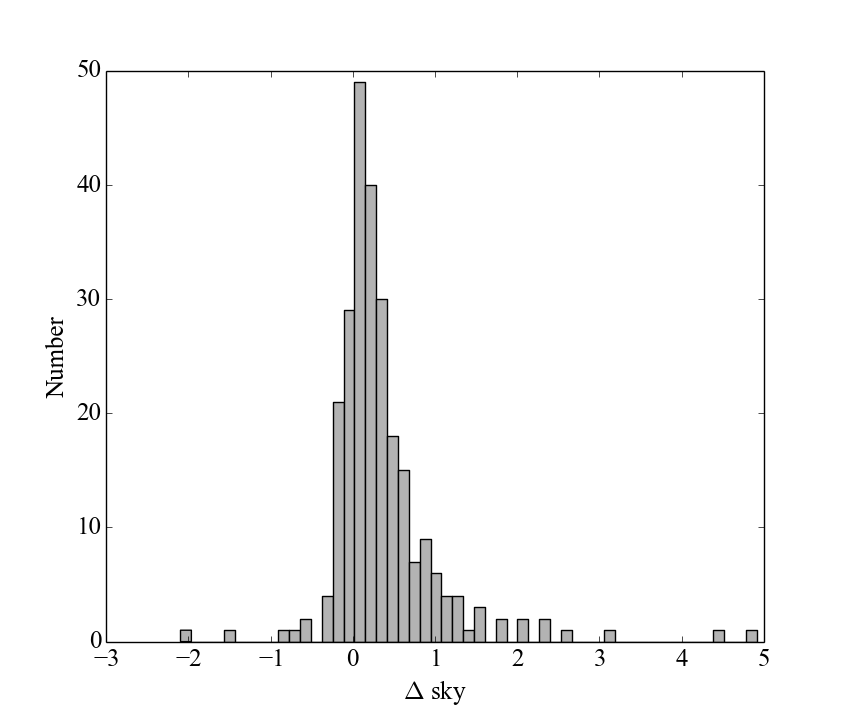
\includegraphics[width=0.7\textwidth]{figs/sky_hist.png}}
	\caption{Histogram of the differences between our sky values and MegaCam/SDSS}
\end{figure}
Sky uncertainty as the standard deviation differs from the pipeline uncertainties ($\sqrt{sky}$) by around 40\%. 

% subsection sky_detection (end)


\subsection{Example Decomposition} % (fold)
\label{sub:example_decompositions}
We present a typical galaxy decomposition and classifications for a disk exhibiting upbending to illustrate the classification process. ID 1237667444048265310 is a typical example of a type-III classified galaxy.

\begin{sidewaysfigure}[p]
	\centering
	\makebox[1.\columnwidth]{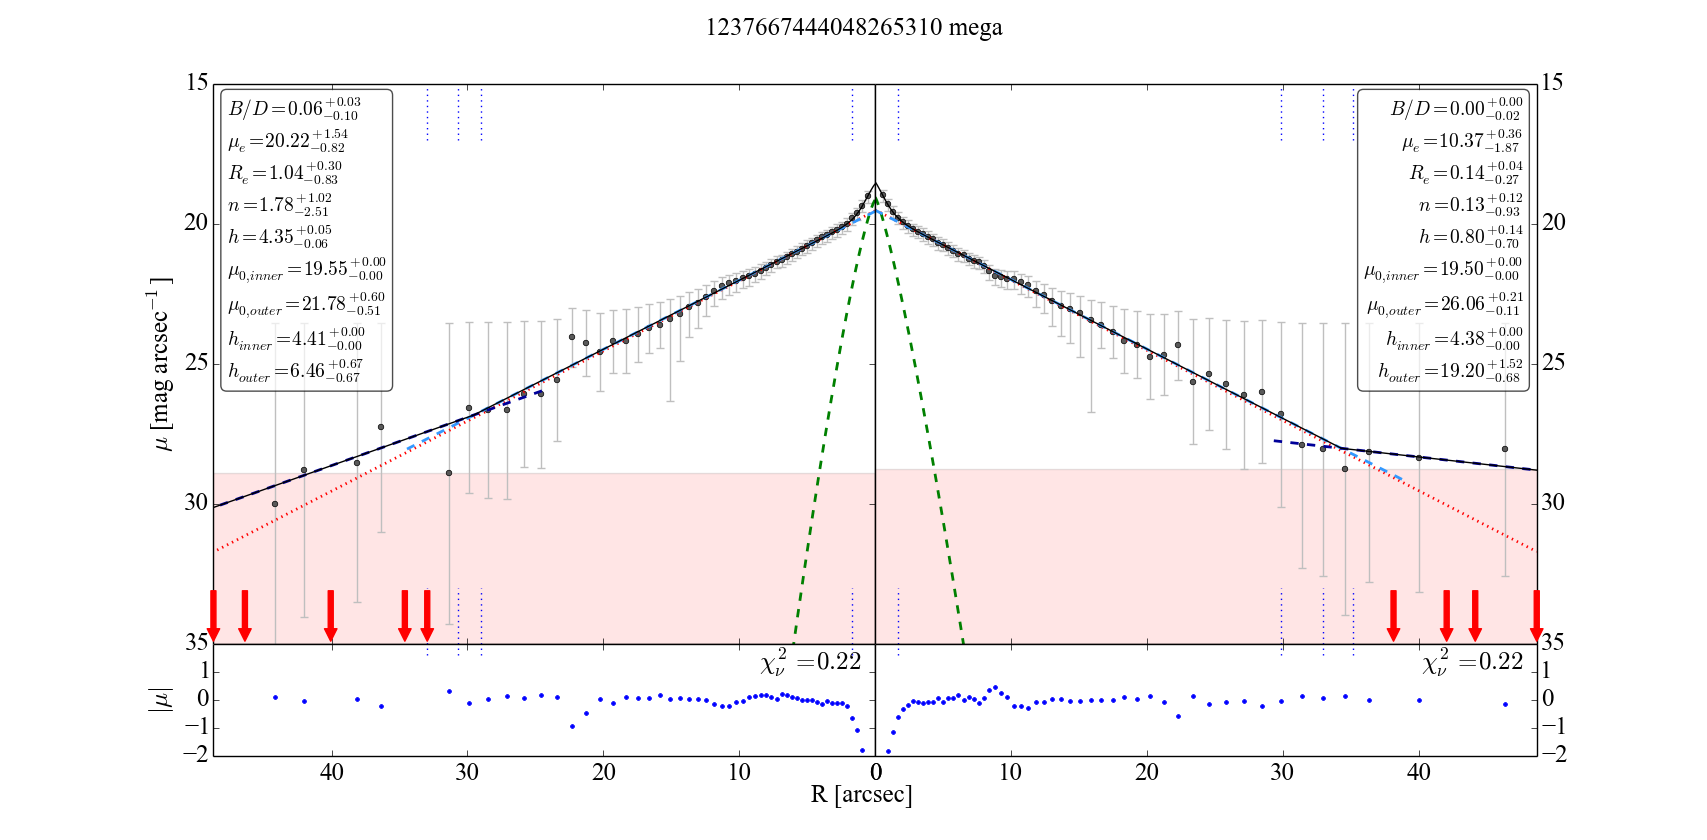
\includegraphics[width=1.5\textwidth]{figs/example_decomp.png}}
	\label{fig: The mega profiles of 1237667444048265310}
	\caption{\footnotesize{The surface brightness profile for the MegaCam image of 1237667444048265310. The plot shows the inner and outer disks in light and dark dashed lines respectively. The bulge is illustrated in green and the original pre-truncated disk is shown as a red dotted line. The total is depicted with a thin black line.
		 Unreal (negative counts) values are shown with red arrows and the critical sky value as the red region. The dashed lines at the top and bottom denote the lower sky limit, lower break limit, upper break limit and bulge cut-off radius, working inwards. Normalised magnitude residuals are shown at the bottom.}}
\end{sidewaysfigure}
\ref{fig: The mega profiles of 1237667444048265310} shows the surface brightness profile of 1237667444048265310. Both MegaCam profiles, representing the different major axes, are completely independently fit. This galaxy is a typical example of an error in truncation detection. Usually there is one profile per galaxy which exhibits this undesirable behaviour. This problem cannot be remedied by restricting the parameters in the fit, since any more restriction tends to yield unreal solutions.

Firstly, a simple bulge + disc is fit to the profile, resulting in a typical profile with a disc scale length of $\sim 6$ arcsec and bulge effective surface brightness of $\sim 20$ mag. 

On the other hand, the bulge shape -characterised by the \sersic index- varies between SDSS and MegaCam fits. Though this changes the shape of the bulge entirely, its surface brightness remains small enough ($\mu_B < \mu_D + 0.2$ mag) as to not have an impact the total at large $R$.

Next, the automated truncation detection yields a potential break point and the two disks are parameterised. The routine classifies these individual fits as Type-III (upbended) since the lower limit on the outer scale length does not fall below the upper limit on the inner scale length. 

As seen in the residual plot accompanying the fits, there is poor fit at the centre of the galaxy, where the bulge is strongest. Since the truncation fit only subtracts the bulge's contribution to the total magnitude, it is likely that the poor central fit is due to neglection of bulge light.

The next step is to combine the images to yield overall parameters for the entire galaxy. However, although there is a good agreement of pre-truncated-fit -called `classic' from now on- disk parameters between cameras there is a discrepancy in the \sersic index of the bulge. SDSS fits a small $n\approx 0.5$ bulge whilst MegaCam finds an expansive $n\approx 1.5$ bulge. 

This discrepancy error is a major problem when combining results as averaging the parameters does not yield an accurate `one-size-fits-all' solution. We proceed by combining their bootstraps instead. This does not solve the problem of not yielding an accurate solution but it does provide an accurate error on the result, unlike a weighted arithmetic mean \citep{andrae_error_2010}. 

Defining the truncation strength as 
\begin{equation}
	S_h =  \frac{h_{outer} - h_{inner}}{h_{inner}},
\end{equation}
we find that $S_h = 1.3^{+0.9}_{-0.7} > 0$ for the combined profile and so is classified as Type-III.


% \begin{tabular}[cccc]
	% table of combined fit parameters
% \end{tabular}

% subsection example_decompositions (end)

\subsection{Sample Properties}
Though all profiles have been successfully fit with a disk dominated outer profile, it was not always real. There were frequent situations where a disc with perturbation (Allen type-6) were fit. These galaxies usually had what appears to be previously unseen spiral patterns, wide bars or simply a bulge dominated outer profile. Since these components are not part of this investigation, these galaxies were discarded.

The initial sample of profiles was also filtered by removing galaxies whose profiles yield hugely disagreeing results. This was done by eye and the sample was refined to 66 reasonable fits. 

Our sample exhibits a range of bulge sizes, showing that our restrictions on bulge parameters relative to the disk has had little impact on the diversity of our sample. It has even permitted bulge-dominated galaxies with $B/D \approx 0.8$, though even they are still dominated by a disk at large $R$.

\begin{sidewaysfigure}[p]
	\makebox[1.\columnwidth]{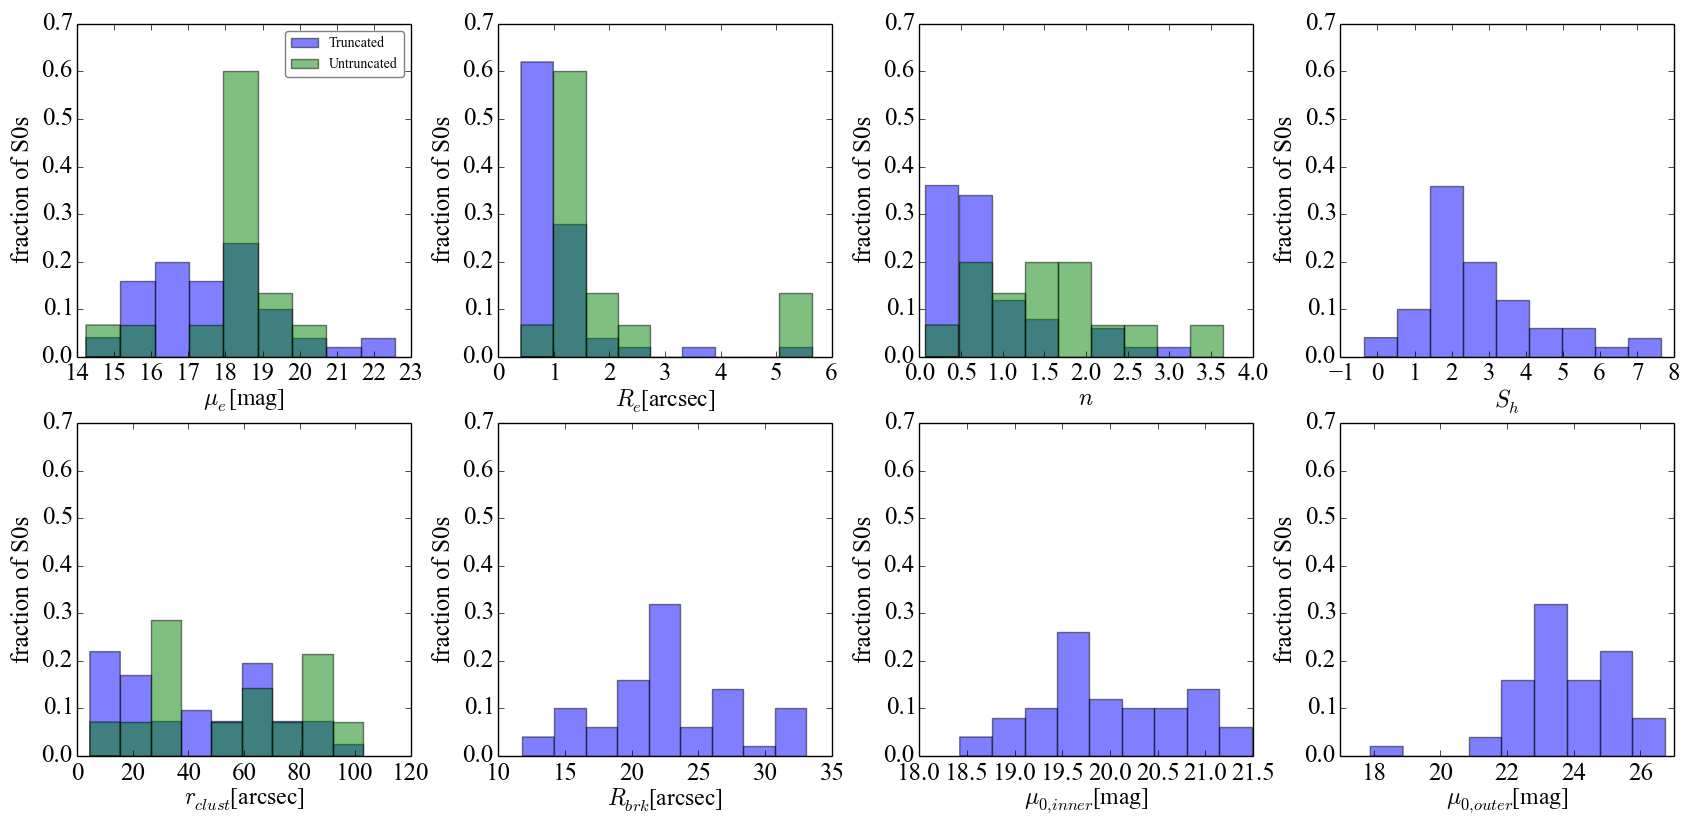
\includegraphics[width=1.\textwidth]{figs/props_hist.png}}
	\caption{Proportion of both truncated and untruncated disks as a function of various parameters where available}
	\label{fig: prop_hist}
\end{sidewaysfigure}

% \begin{tabular}
	% table for truncated and untruncated mean values for parameters
% \end{tabular}

In Type-III disks, the central surface brightness of the outer disk must be greater than that of the inner disk. This can clearly be seen in the sharp divide between the distributions above. Although type-Is and type-IIIs share a similar distribution of effective bulge radii, higher \sersic indices are more frequent in type-I disks. The type-III preference for a more centralised bulge suggests that the upbending is not due to bulge influence which earlier may have escaped notice. 

In truncated galaxies, the break point takes a wide range of radii and the strength of the break exhibits a peak at 2. The small number of truncated galaxies with low break strength can be attributed to the classification process, since a low break strength is more likely to lie within $\sim 1\sigma$ of the classical disk and hence classified as untruncated. 

% subsection Sample Properties (end)

\subsection{Correlations with distance from cluster centre} % (fold)
\label{sub:correlations}
We found no statistically significant evidence of a trend between distance from cluster centre and bulge and classical disk parameters . However, there is a parabolic region of $30 \lesssim R_{clust} \lesssim 60$ arcsecs, $28 \lesssim \mu_{0,outer} \lesssim 25$ mag in which there are no truncated galaxies.

We found evidence of a weak trend between the bulge magnitude and the break radius. A Pearson correlation coefficient of 0.26 indicates an increase in bulge magnitude as the break appears further out in $R$.
\begin{figure}[h]
	\centering
	\label{bulge/break correlation}
	\makebox[0.8\columnwidth]{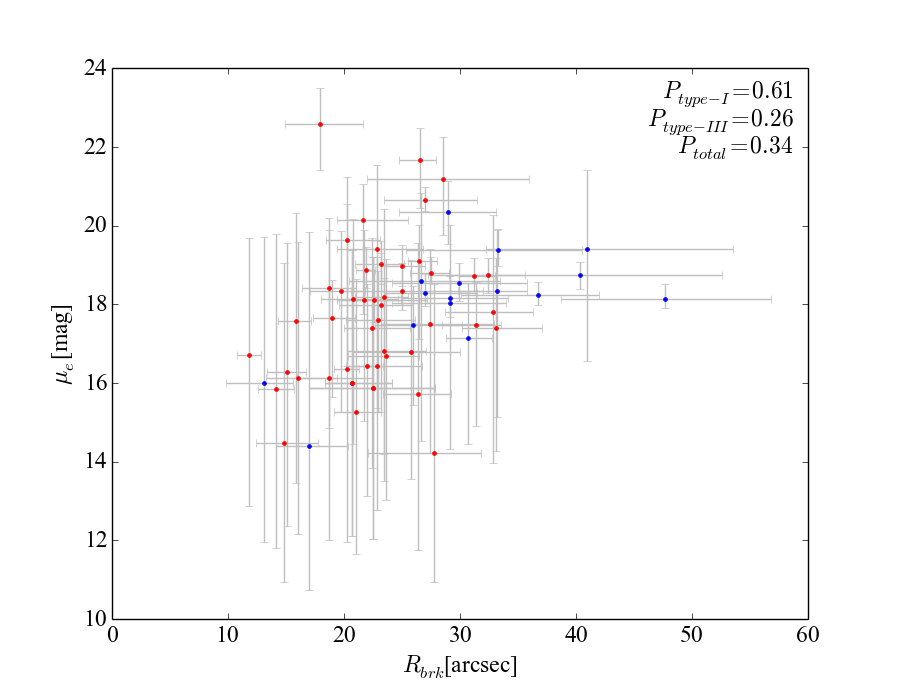
\includegraphics[width=0.8\textwidth]{figs/bulge_mag_vs_brk.png}}
	\caption{\footnotesize{A correlation plot between effective bulge magnitude $\mu_e$ and break radius $R_{brk}$ with truncated galaxies shown in red and untruncated galaxies shown in blue for comparison.}}
\end{figure}
Type-I S0s exhibit a tighter correlation between their potential break radius and bulge magnitude. This demonstrates that this trend is likely an artefact of the fitting process.

\begin{figure}[h]
	\centering
	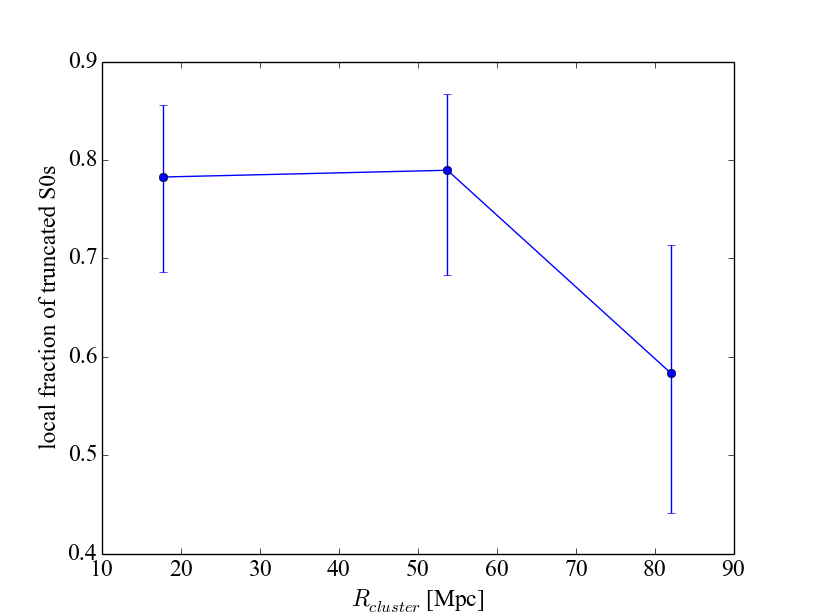
\includegraphics[scale=0.5]{figs/fraction_vs_cluster_radius}
	\caption{Fraction of upbended S0s binned with equal distance bins}
	\label{fraction vs dist}
\end{figure}

A weak trend in fraction of type-III against cluster-centric radius is observed when binning the galaxies into inner, outer and intermediate radii (see \ref{fraction vs dist}. The fraction of truncated S0s at the outskirts ($R > 60 $Mpc) is much lower than that of the innermost region.

% subsection correlations (end)
